\section{OpenFace}
\label{OpenFace}
Ein Open-Source Echtzeitverfahren auf Basis von CLNF für die Bestimmung und Analyse von Gesichtsmerkmalen in Graubildern und Videos. Dabei stehen für diese Anwendung nur die Kameraparameter zur Verfügung und keinerlei Zusätze wie ein Tiefenbild (kann mitverwendet werden wenn es vorhanden ist) oder Infrarotbeleuchtung der Szene.\\
OpenFace kann 68 Landmarks ermitteln, die das Gesicht beschreiben, und mit deren Hilfe Position, Blickrichtung und Gesichtsmerkmale zu bestimmen. Sollte ein Video als Quelle fungieren, kann OpenFace auch lernen, wodurch eine zuverlässigere Verarbeitung erzielt werden kann.\\
Als Ergebnis ist die Kopfposition (Translation und Orientierung) sowie Blickrichtung von Interesse, da mit ihnen zurückrechnet werden kann wohin die Person schaut.\\
Der Rechenaufwand zur Verarbeitung des Eingabebildes ist so ausgelegt, das ein Webcam-Video in Echtzeit ausgewertet werden kann, dies ist im aktuellen Fall nicht notwendig, da es sich um eine nachträgliche Auswertung handelt, bei der es vor allem um Genauigkeit geht.
\subsection{Bestimmung der Landmarks}
\label{bestimmung_Landmarks}
Für die Bestimmung der Landmarks wird OpenFace auf den zuvor bestimmten Bildausschnitten eingesetzt. Dies bietet mehrere Vorteile, so wird nur auf Bildbereichen gearbeitet, in denen ein Gesicht zu sehen ist und unnötige Suche vermieden. Außerdem kann für jede Person die passende Initialisierung des CLNF, basierend auf dem letzten Ergebnis dieser Person, gewählt werden, auch für jene Personen die nur selten dargestellt sind. Auf diese Weise kann der Bildausschnitt möglichst exakt und gleichzeitig mit den anderen ausgewertet werden.\\
Für die eigentliche Bestimmung der Landmarks bietet OpenFace zwei verschiedene Methoden, die Berechnung auf Bildern und Videos. Der Hauptunterschied ist das Lernen, dass bei der Videoauswertung verwendet wird, wodurch sich der Toleranzbereich deutlich erhöht und bessere Ergebnisse liefert werden. Dies liegt an der Anpassung des Modells und dem möglichen Tracking der Landmarks.\\
Dies ist Interessant für die spätere Anwendung, da somit auch Einzelbilder verwendet werden können, die eine deutlich höhere Auflösung besitzen als ein Video. Allerdings haben die Vorabtestes (\autoref{Vorversuche}), gezeigt, das bei Verwendung von Einzelbilder der maximale Winkel relativ zur Kamera beträchtlich sinkt. Außerdem hat sich gezeigt das bei Verwendung eines Videos das Gesicht deutlich kleiner dargestellt sein kann bis keine Auswertung mehr möglich ist. Sollte ein Gesicht im aktuellen Frame erfolgreichen detektiert werden, können auch die nachfolgenden Frames durch das Lernen ausgewertet werden.\\
Dennoch kann es passieren, dass trotz allem ein Gesicht falsch detektiert wird, wie z.B. das Erkennen eines sehr kleinen Gesichtes innerhalb einer Ohrmuschel. In solch einem Fall muss das CLNF zurückgesetzt werden, damit sich der Fehler nicht fortpflanzt.
\subsubsection{Gesichts-Landmarks: Detektion und Verfolgung}
Für die Bestimmung und Tracking der Landmarks wird ein Conditional Local Neural Fields (CLNF) eingesetzt. Dabei Handels es sich im Grunde um ein Constrained Local Model (CLM) nur mit verbesserter Patch Experts und Optimierungsfunktionen.\\
Die beiden Hauptkomponenten des CLNF von OpenFace ist das Point Distribution Model (PDM) zur Erfassung der Anordnung der Landmarks und Patch Experts zum Erfassen der Variante der einzelnen Landmarks.\\
Zu Beginn werden verschiedene initiale Hypothesen aus der dlib-Bibliothek verwendet und die Passende zur Eingabe ausgewählt. Bei den unterschiedlichen initial Hypothesen handelt es sich um die Darstellung verschiedener Gesichtsorientierungen auf denen unterschiedliche Netze trainiert wurden. Dies Herangehensweise ist langsam, aber auch exakter als eine einfache Hypothese. Wird ein Tracing, das Verfolgen der Landmarks über mehrere Frames, durchgeführt wird als initiale Hypothese das Ergebnis aus der letzten Eingabe verwendet. Sollte das Tracing scheitern, wird das CNN reseted um Neu zu beginnen mit den ursprünglichen Hypothesen.\\
Auf diese Weise werden 68 Gesichts-Landmarks und  weitere 28 pro Auge erfasst. Zur Berechnung auf den Gesichtern sollten diese laut Paper \cite{OpenFace} eine Optimalgröße von 100 Pixeln für eine zuverlässige Detektion aufweisen.
\subsubsection{Erkennen der Gesichtsmerkmale}
Dieser Schritt kann von OpenFace ausgeführt werden, ist aber im aktuellen Fall nicht von Relevanz, da die Blickrichtung von Interesse ist und nicht die Mimik der Probanden.
\subsubsection{Veröffentlichte Genauigkeit der Kopforientierung}
Um die Qualität der Berechnung auf dem Kopf zu bewerten wurde im Paper \cite{OpenFace} der \glqq Biwi Kinect head pose\grqq \cite{BIWI_database},\glqq ICT-3DHP\grqq \cite{ICT_database} und \glqq BU Datensatz\grqq \cite{BU_database} ausgewertet. Dabei handelt es sich um Portrait-Fotos von Probanden, deren Körper in Richtung Kamera ausgerichtet sind und ihren Kopf in eine beliebige Richtung drehen. Für die Genauigkeit der Kopfposition haben sich Werte ergeben in Grad, siehe \autoref{OpenFace_Error}.\\
Für die Qualität zur Bestimmung der Blickrichtung wurde der Augendatensatz \glqq Appearancebased gaze estimation in the wild\grqq \cite{database_Eye_old} zur Bestimmung der Blickrichtung verwendet und es ergab sich ein durchschnittlichen Fehler von $9,96$ Grad.
\begin{figure}[h]
	\centering
	\begin{tabular}{|l|c|c|c||c|c|}
		\hline
		&Yaw&Pitch&Roll&Mean&Median\\\hline
		Biwi Kinect&7.9&5.6&4.5&6.0&2.6\\\hline
		BU dataset&2.8&3.3&2.3&2.8&2.0\\\hline
		ICT-3DHP&3.6&3.6&3.6&3.6&-\\\hline
	\end{tabular}
	\caption{Veröffentlichte Abweichung von OpenFace auf verschiedenen Datensätze.\cite{OpenFace}}
	\label{OpenFace_Error}
\end{figure}
\subsection{Bestimmung des Arbeitsbereiches}
Da mit diesem Verfahren die Landmarks bestimmt werden, aus denen die Gesichtsorientierung abgeleitet wird, sollen die Grenzen dieses Verfahrens ermittelt werden. Von Interesse ist die Bildqualität in der ein Gesicht dargestellt werden muss um dieses noch verarbeiten zu können und wie sehr diese Person von der Kamera abgewandt sein kann.
\subsubsection{Auswirkung der Auflösung auf die Detektionsrate}
Durch die Aufgabenstellung muss das Verfahren zuverlässig bezüglich der Distanzen bzw. Darstellungsgröße sein. Zur Messung wurde der Datensatz von Labeled Faces in the Wild \cite{database_Face} verwendet. In diesem Datensatz ergibt sich im Originalbild eine durchschnittliche Kopfbreite von 94 Pixel. Bei Random Forests for Real Time 3D Face Analysis \cite{database_Face_Ori} ist die durchschnittliche Breite 78 Pixel.\\
Zur Durchführung wurden die Bildgröße mit dem Skalierungsfaktor multipliziert und linear verkleinert um so kleinere, weiter entferntere Gesichter zu simulieren und anschließend mit dem Image-Detector von OpenFace verarbeitet. Das Ergebnis ist in \autoref{img_lineareverkleinerung} dargestellt.\\
Es ist zu erkennen, dass die Wahrscheinlichkeit auf eine erfolgreiche Detektion ab einer Skalierung von $0,6$ bei BIWI auf dem, also Gesichert mit etwa 47 Pixel Breite, rapide abnimmt. Bei der in \autoref{hardware} beschriebenen Kamera entspricht dies einer Distanz von etwa $4,5m$.\\
Bei der maximalen Distanz auf der gearbeitet werden soll $(8m)$ ergibt sich eine Gesichtsgröße von etwa 22 Pixel, das einer Skalierung von $0,25$ entspricht. Bei dieser Bildgröße ist in der Standardanwendung ohne Skalierung keine Detektion möglich, siehe \autoref{img_lineareverkleinerung}.
\begin{figure}
	\centering
	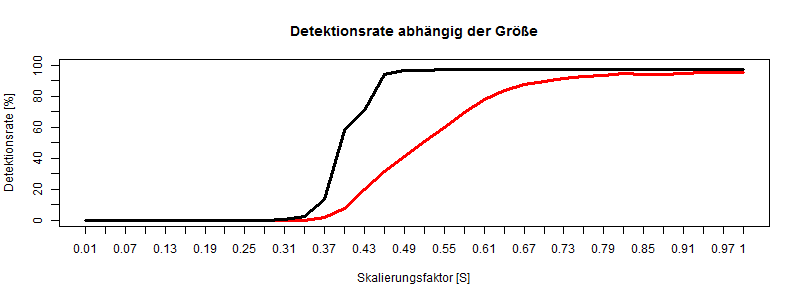
\includegraphics[width=\linewidth]{img_Skalierung/Gesicht_Rate}
	\caption{Die Bilder aus Labeled Faces in the Wild \cite{database_Face} (schwarz) und Biwi Kinect Head Pose Database \cite{BIWI_database} (grau) wurden mit den Faktor auf der X-Achse linear verkleinert und die Erkennungsrate Y-Achse abgebildet}
	\label{img_lineareverkleinerung}
\end{figure}
\subsubsection{Auswirkung der verschiedenen Skalierungesverfahren auf die Detektion}
\label{OpenFace_skal}
Um die Auswirkung der Skalierungsverfahren zu bestimmen, wurden verschiedene Gesichtsgrößen simuliert, indem sie um den angegeben Faktor linear verkleinert wurden.\\
Beim Random Forest Datensatz \cite{database_Face_Ori} werden nur jene Bilder ausgewertet, in denen OpenFace bei einem Vorabtest ein Gesicht erkannte und nur der entsprechende Bildbereich ausgewertet. Als Zielgröße bei der Skalierung wurde das $1,3$ fache der Originalgröße gesetzt, damit die abgebildeten Gesichter in etwa 100 Pixel groß sind für die Auswertung. Zur Berechnungen wurde eine Brennweite von $531,15$ angenommen.\\
Bei dem Labeld Face in the Wild \cite{database_Face} Datensatz wurden alle Bilder im Orginal verwendet, um den angegebenen Skalierungsfaktor verkleinert und mit dem angegebenen Verfahren wieder auf die Orginalgröße gebracht.\\
Die Auswirkung der verschiedenen Skalierungsverfahren auf die Detektionswahrscheinlichkeit ist in \autoref{img_hochskalliern} dargestellt.\\
Es ist zu erkennen das die Detektionsrate über einen weiten Bereich, $[1;0,25]$ bei der Skalierung, nur sehr wenig abnimmt. Durch die Vergrößerung können somit jene Gesichter in Bereichen die normal nicht erkennbar sind, ausgewertet werden.\\
Erst bei den sehr kleinen Skalierungen ist ein wirklicher unterschied zwischen den Verfahren zu erkennen. So nimmt die Detektionsrate bei  Nearest-Neighbor (rot) deutlich früher ab als bei den anderen verfahren. Das Bicubic (blau) und Lanczos (grün) Verfahren haben die höchste Detektionsrate und fallen auch am spätestens ab, wobei Bicubic minimal besser ausfällt.\\
Es zeigt sich, das durch die Skalierung die Anforderungen auf eine Detektion von Gesichtern mit 22 Pixel (Skalierung $0,25$, $8m$), von allen Verfahren erfüllt.\\
Ausgehend vom Skalierungsfaktor des Bicubic-Verfahren ab welchem die Detektionsrate stark abfällt, wären Distanzen bis zu $14m$ möglich (Basierend auf der Auflösung der Actioncam).\\
Allerdings ist das Bild durch die Verkleinerung deutlich besser als bei Originalaufnahmen, da Pixelrauschen und Ähnliches nicht vorhanden ist.
\begin{figure}
	\centering
	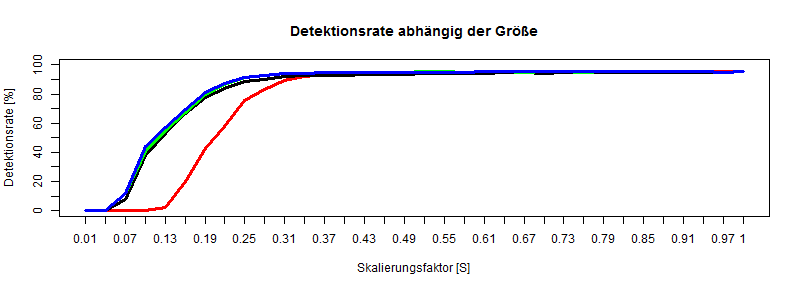
\includegraphics[width=\linewidth]{img_Skalierung/Resize_Rate_Ges}\\
	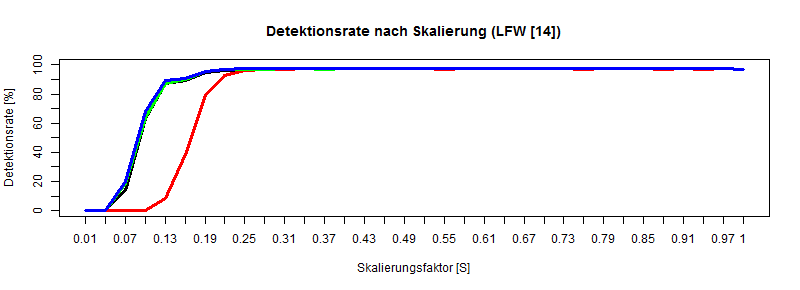
\includegraphics[width=\linewidth]{img_Skalierung/Resize_Rate_lfw}
	\caption{Die Bilder wurden mit den Faktor auf der X-Achse linear verkleinert und mit den verschiedenen Verfahren wieder vergrößert \autoref{scale_Algos}. Aufgetragen gegen die Y-Achse ist die  Detektionswahrscheinlichkeit.\\
	Bicubic (blau), Lanczos (grün), Linear (schwarz), Nearest-Neighbor (rot)\\
	Oben: Biwi Kinect Head Pose Database \cite{BIWI_database}\\
	Unten: Labeled Faces in the Wild\cite{database_Face}}
	\label{img_hochskalliern}
\end{figure}
\subsubsection{Arbeitsbereich bezüglich Rotation}
In \autoref{img_Rot_Dif} ist der Median der Differenz zwischen den berechneten Winkel von PoseWorld und der Angabe im Datensatz dargestellt.\\
Bei der X-Rotation zeigt sich, dass das Bicubic-Verfahren im Vergleich zu den anderen 1 Grad schlechter abschneidet. Der Fehler von Lanczos, Linear und Nearest-Neighbor liegt bei etwa $19^\circ$ bis zu einer Skalierung von $0,25$.\\
Es Zeigt sich, das der Median in den Abweichung auf der Y-Achse (nicken) sehr hoch ausfällt mit knapp über $25^\circ$. 
Dabei liefern alle vier Verfahren nahezu identische Ergebnisse, die auch konstant bleiben bezüglich der Skalierung.\\
Die Z-Rotation wird am besten bestimmt mit einer Abweichung von etwa $7,5^\circ$, dabei ist aber auch zu beachten Wertebereich geringer als bei den anderen beiden Rotationen.
Hier liefert Bicubic das Beste Ergebnis, wobei der unterschied weniger als ein halbes Grad beträgt.\\
Für alle Berechnungen zeigt sich, das der Fehler konstant bleibt, bis zu der Skalierung von $0.25$, bei der auch Detektion scheitert.\\
Neben der Qualität von den bestimmten Winkel, ist auch der Arbeitsbereich von Interesse in dem Gesichter bei verschiedenen Skalierungen noch erkannt werden können. Da ein Gesicht das außerhalb dieser Bereiche liegt nicht erkannt und ausgewertet werden kann.\\
In \autoref{img_Rot_Max} sind die Quantile bei $50\%;80\%;99,5\%$ und der Maximalwert, von den Rotationswinkel der Bilder aus dem Biwi Kinect Head Pose Database \cite{BIWI_database} ein Gesicht erkannt wurde, abgebildet. Durch den großen Unterschied zwischen den $80\%$-Wert, ;$99,5\%$-Wert und dem Maximalwert legt die Vermutung nahe, dass es sich bei diesen Werten um falsch detektierte Bilder handelt, aber eine Rotation des Kopfe von $45\%$ in alle Richtungen erkannt und ausgewertet werden kann.\\
Eine genaue Darstellung der Messung ist in \autoref{Abbildungen} abgebildet, für die X-Rotation \autoref{img_X_Rot_Skal}, Y-Rotation \autoref{img_Y_Rot_Skal} und Z-Rotation \autoref{img_Z_Rot_Skal}.
\begin{figure}
	\centering
	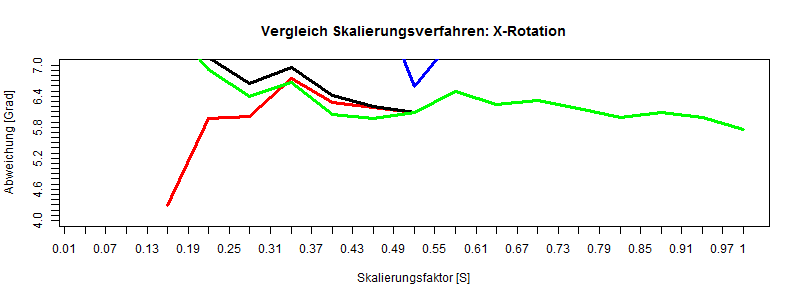
\includegraphics[width=\linewidth]{img_Skalierung/Skal_Diff_RX}
	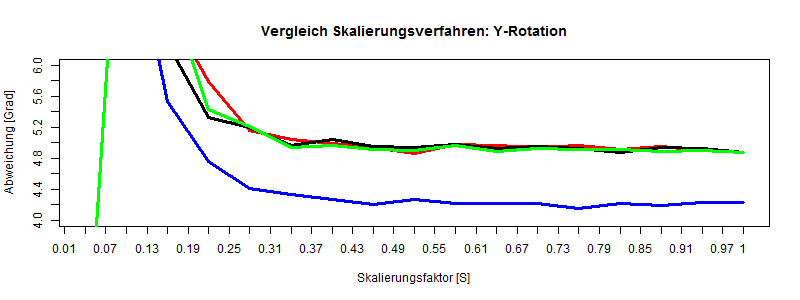
\includegraphics[width=\linewidth]{img_Skalierung/Skal_Diff_RY}
	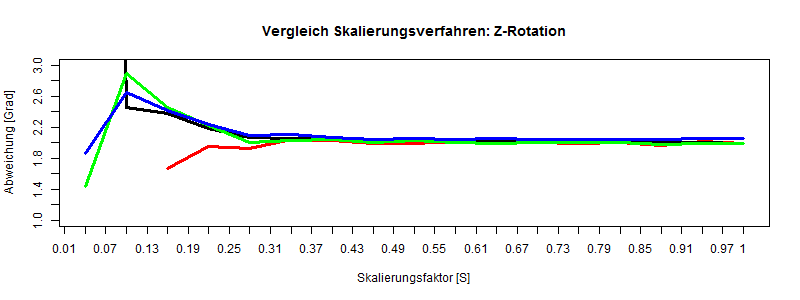
\includegraphics[width=\linewidth]{img_Skalierung/Skal_Diff_RZ}
	\caption{Dargestellt ist der Median der Abweichung zwischen der Berechneten Drehung und der des Datensatzes.\\
		Bicubic (blau), Lanczos (grün), Linear (schwarz), Nearest-Neighbor (rot)\\
		Oben: X-Rotation Wertebereich: $[18;21]^\circ$\\
		Mitte: Y-Rotation Wertebereich: $[24;27]^\circ$\\
		Unten: Z-Rotation Wertebereich: $[6;9]^\circ$}
	\label{img_Rot_Dif}
\end{figure}
\subsubsection{Auswirkung der Skalierungsverfahren auf die Positinsbestimmung}
Für eine zuverlässige Auswertung ist auch die Bestimmung der Position von Interesse. Im Biwi Kinect Head Pose Database \cite{BIWI_database} ist die Durchschnittliche Distanz zwischen Kamera und Proband bei etwas $90cm$. Der Median der Differenz zwischen Datensatz und Rechnung ist in \autoref{img_Pos_Dif} dargestellt. Bei sehr kleinen Skalierungen existieren durchaus auch sehr große Fehler, diese wurden allerdings bei der Darstellung abgeschnitten, da bei dieser Größe die Detektionsrate so klein ist, dass sie nahezu irrelevant werden.\\
Es Zeigt sich, das die Position in horizontaler und vertikaler Richtung auf etwa $6,5cm$ genau bestimmt werden kann, die Distanz (Tiefe) auf $9cm$ und auch au sehr klein Skalierten Bildern.\\
Nearest-Neighbor hat bei der Berechnung der X-Position die geringste Abweichung zu den anderen getesteten Verfahren mit $6,37cm$ bei der Originalgröße.\\
Bei der Bestimmung der Y-Position, liefern alle Skalierungsverfahren sehr ähnlich Ergebnisse mit einem Fehler von $6,5cm$, wobei das lineare Verfahren minimal besser ausfällt bei kleinen Skalierungen.\\
Die größte Ungenauigkeit liegt bei der Z-Position (Tiefe). Das Lineare Verfahren liefert auch hier das beste Ergebnis, mit einer Abweichung von $8,92cm$, dabei ist der Unterschied zu den anderen Verfahren minimal.\\
Eine ausführliche Darstellung der Messung ist in \autoref{img_X_Pos_Skal}, \autoref{img_Y_Pos_Skal} und \autoref{img_Z_Pos_Skal} dargestellt
\begin{figure}
	\centering
	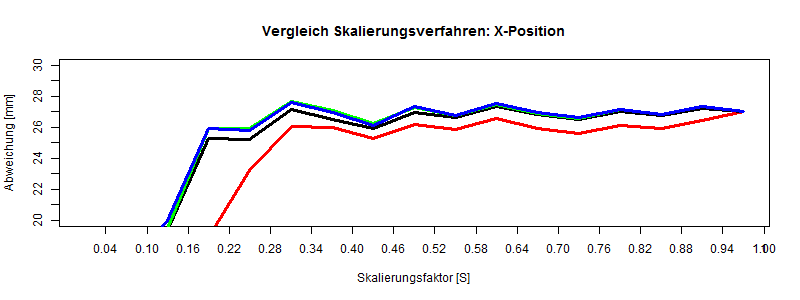
\includegraphics[width=\linewidth]{img_Skalierung/Skal_Diff_TX}
	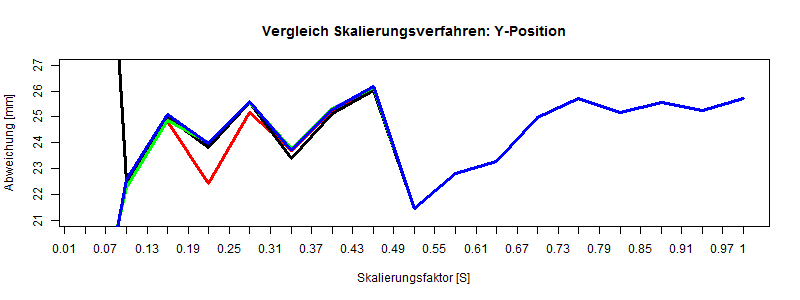
\includegraphics[width=\linewidth]{img_Skalierung/Skal_Diff_TY}
	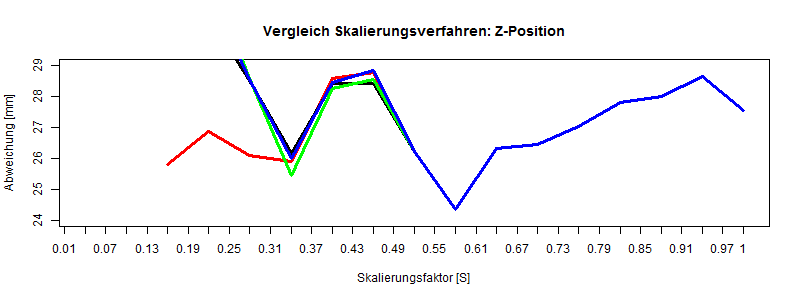
\includegraphics[width=\linewidth]{img_Skalierung/Skal_Diff_TZ}
	\caption{Dargestellt ist der Median der Abweichung zwischen der Berechneten Drehung und der des Datensatzes.\\
		Bicubic (blau), Lanczos (grün), Linear (schwarz), Nearest-Neighbor (rot)\\
		Oben: X-Position Abweichung: $62-68mm$\\
		Mitte: Y-Position Abweichung: $58-68mm$\\
		Unten: Z-Position Abweichung: $66-90mm$}
	\label{img_Pos_Dif}
\end{figure}
\subsubsection{Auswirkung von Pixelrauschen auf die Detektion}
Mit diesem Test soll geprüft werden, welches der Verfahren auch stabil gegenüber Rauschen ist.\\
Um Pixelrauchen zu simulieren, wurden die Bilder aus Labeled Faces in the Wild \cite{database_Face} entsprechend verkleinert, mit Rauschen versehen um sie anschließend mit den unterschiedlichen Verfahren zu vergrößern.\\
Das Rauschen wird für jedes Pixel simuliert, indem eine Wahrscheinlichkeit von $50\%$ besteht auf eine gleich verteilte Abweichung von $\pm 10\%$ des Originalen Farbwertes. Dieser Vorgag wurde für jedes Bild viermal wiederholt um Zufälligkeiten bei der Rauschsimulation zu vermeiden.\\
Wie zu erwarten ist Nearest-Neighbor am schlechtesten, aber auch zwischen den anderen Verfahren sind nun unterscheiden zu erkennen, siehe \autoref{img_hochskalliern_nois}. Die gesamte Erkrankungsrate ist signifikant kleiner als ohne Rauschen, wobei die Position $(0.15)$, ab welcher die Erkennungsrate rapide abfällt, beibehalten wird.
\begin{figure}
	\centering
 	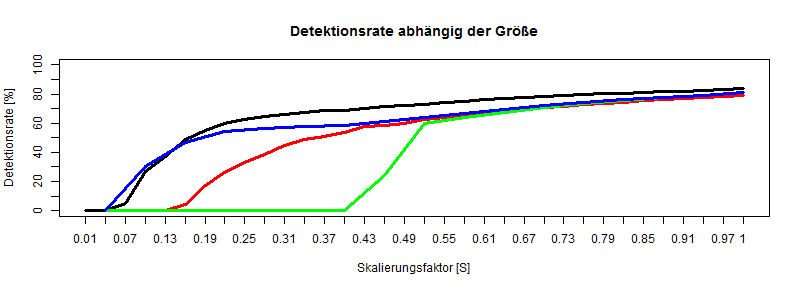
\includegraphics[width=\linewidth]{img_Skalierung/Hochskalliern_Nois}
	\caption{Bilder aus Labeled Faces in the Wild \cite{database_Face}, mit dem X-Faktor verkleinert, um jedes Pixel mit $50\%$ Wahrscheinlichkeit auf $\pm 10\%$ Gleichverteilung der Abweichung}
	\label{img_hochskalliern_nois}
\end{figure}
\subsection{Ergebnis bezüglich Verwendbarkeit}
Anhand der Detektionsrate abhängig von der Skalierung, siehe \autoref{img_lineareverkleinerung}, kann entnommen werden, das Gesichter unter 50 Pixel Größe nicht mehr sinnvoll erkannt werden können.\\
Werden sie hingegen hochskaliert, können sogar Gesichter mit einer Größe von 25 Pixel gefunden werde. Dies bedeutet das mit diesem Trick auch mit der Hälfte des Informationsgehaltes noch gearbeitet werden, wenn sie dadurch dem Trainingsdatensatze eher entsprechen.\\
Die Lanczos-Skalierung hat im Test mit einfach verkleinerten Bilder am Besten abgeschnitten mit einer der höchsten Detektionsrate bei den Skalierungen. Auch Bei der Bestimmung der Rotation gehört es zu den besten Verfahren und kann auch bei der Positionsbestimmung überzeugen. Alle Anderen Verfahren zeigen schwächen, wie die deutlich früheren Abfall der Detektionsrate von Nearest-Neighbor, die im Verhältnis zu den anderen starken Abweichung der X-Rotation von Bicubic oder das in allen Bereichen leicht schlechter abzuschneidende Lineare-Verfahren als das jeweilig beste.\\
Der Test mit dem Pixelrauschen sollen etwaige Bildfehler simulieren, wie es bei schlechten Kameras der Fall sein kann und die Auswertung auf kleinen Bildausschnitten erschwert. Somit kann auch gezeigt werden das dieser Trick mit der Vergrößerung auch sehr wahrscheinlich in der späteren Anwendung funktionieren wird.\\
Es zeigt sich auch, dass für die Skalierung das Lineare verfahren verwendet werden soll, da mit diesem im Verrauschen Bild die höchste Detektionsrate erreicht wird. Da die Unterschiede zwischen den einzelnen Verfahren aber recht gering ausfallen kann die Wahl des Skalierungsverfahren durch andere Kriterien abhängig gemacht werden wie z.B. der Rechenzeit, wobei vom Nearest-Neighbor abgeraten werden kann.